\chapter{¿Qué es un dron y cómo vuela?}

\begin{enpocas}
Las partes de un cuadrirrotor, por qué vuela, cómo sube, avanza y gira con solo cambiar la velocidad
de sus cuatro motores, y cómo es el Tarot 650 que usamos.
\end{enpocas}

\section{Drones, multirrotores y cuadrirrotores}

``Dron'' es el nombre popular de un \textbf{vehículo aéreo no tripulado} (UAV, por sus siglas en
inglés): una aeronave sin piloto a bordo. Puede ser un avión de ala fija, un helicóptero o, el caso
más común, un \textbf{multirrotor}: una aeronave con varias hélices horizontales. El de cuatro
hélices se llama \textbf{cuadrirrotor} o \textbf{cuadricóptero}.

¿Por qué cuatro? Porque es el número mínimo con el que se puede controlar todo el movimiento sin
piezas móviles más que los propios motores: no hay alerones, timones ni ``plato cíclico'' como en
un helicóptero. Eso los hace baratos, robustos y fáciles de reparar; a cambio, son inestables por
naturaleza: sin una computadora que corrija cientos de veces por segundo, se voltean.

\begin{recuerda}
Un cuadrirrotor no tiene superficies de control. Todo lo que hace (subir, inclinarse, girar) lo
consigue cambiando la velocidad de sus cuatro motores. Por eso el \emph{control} es el corazón del
dron.
\end{recuerda}

\section{Las partes}

\begin{figure}[H]
\centering
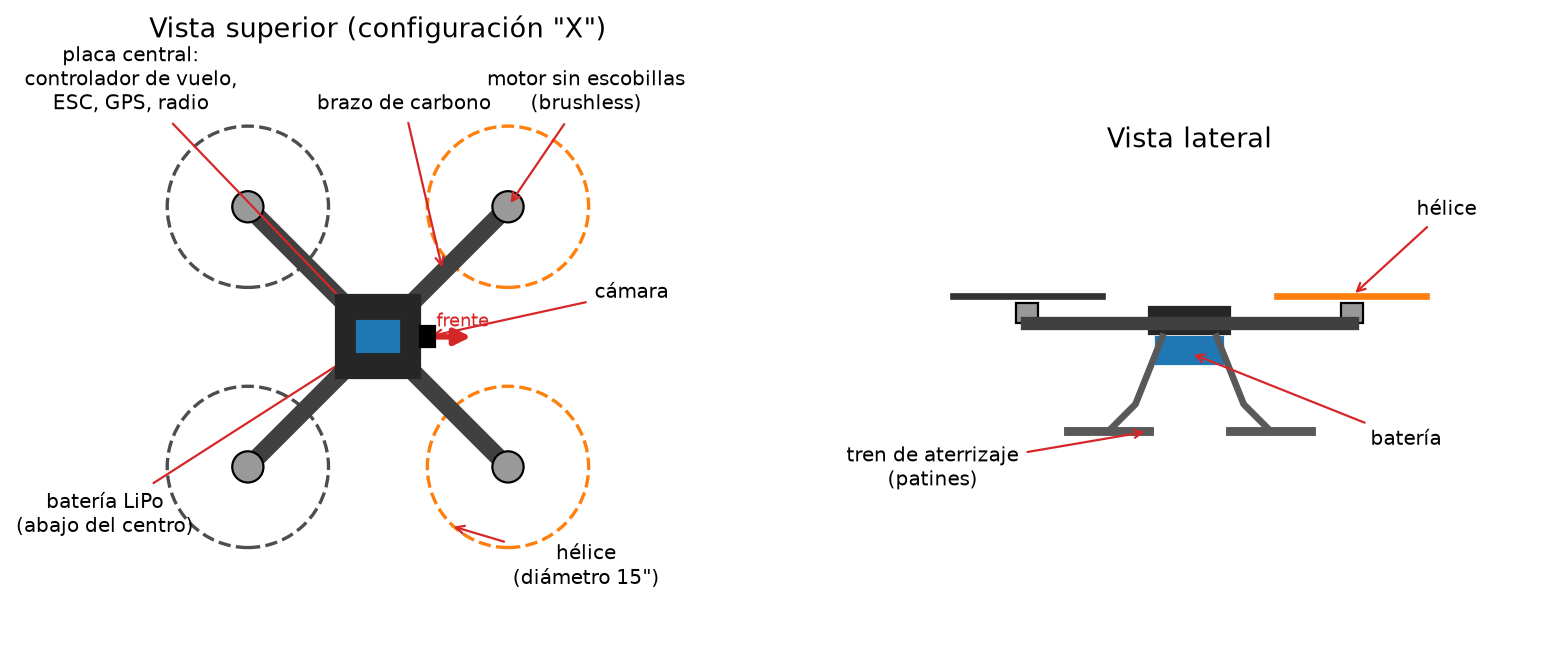
\includegraphics[width=\textwidth]{c_partes.png}
\caption{Partes de un cuadrirrotor como el Tarot 650.}
\label{fig:partes}
\end{figure}

\begin{description}
  \item[Marco (frame).] La estructura: una placa central y cuatro brazos. En el Tarot son de fibra de
        carbono, ligera y rígida. Los brazos del Tarot se pueden plegar para transportarlo.
  \item[Motores sin escobillas (brushless).] Motores eléctricos trifásicos muy eficientes. En el Tarot
        se usan T-Motor MN3508. Su constante KV dice cuántas revoluciones por minuto da por cada volt.
  \item[ESC (controlador electrónico de velocidad).] Uno por motor. Recibe una orden (``gira a tanto'')
        y genera las corrientes trifásicas para lograrlo.
  \item[Hélices.] Convierten el giro en empuje. Se describen con dos números: diámetro y paso, en
        pulgadas. Las del Tarot son de $15\times5$: 15'' de diámetro (38~cm) y 5'' de paso (lo que
        avanzarían en una vuelta si se ``atornillaran'' en el aire).
  \item[Batería LiPo.] Polímero de litio: mucha energía para su peso. Se describen por el número de
        celdas en serie (4S, 6S: 3.7~V cada una) y su capacidad en mAh.
  \item[Controlador de vuelo.] La computadora a bordo: lee los sensores y decide la velocidad de cada
        motor cientos de veces por segundo. Puede llevar ArduPilot o PX4. En nuestra simulación ese
        papel lo hacen nuestros controladores en Python o ArduPilot en SITL.
  \item[Sensores.] IMU (acelerómetros y giroscopios: cómo se mueve y gira), barómetro (altura),
        magnetómetro (brújula), GPS (posición) y, según la misión, cámaras y LiDAR.
  \item[Tren de aterrizaje.] Patas o patines para posarse sin dañar la cámara ni la batería.
\end{description}

\section{¿Por qué vuela? El empuje}

Una hélice que gira empuja aire hacia abajo; por la tercera ley de Newton (acción y reacción), el
aire empuja a la hélice hacia arriba. A esa fuerza se le llama \textbf{empuje}. Crece con el
\emph{cuadrado} de la velocidad de giro: al doble de velocidad, cuatro veces más empuje.

\begin{figure}[H]
\centering
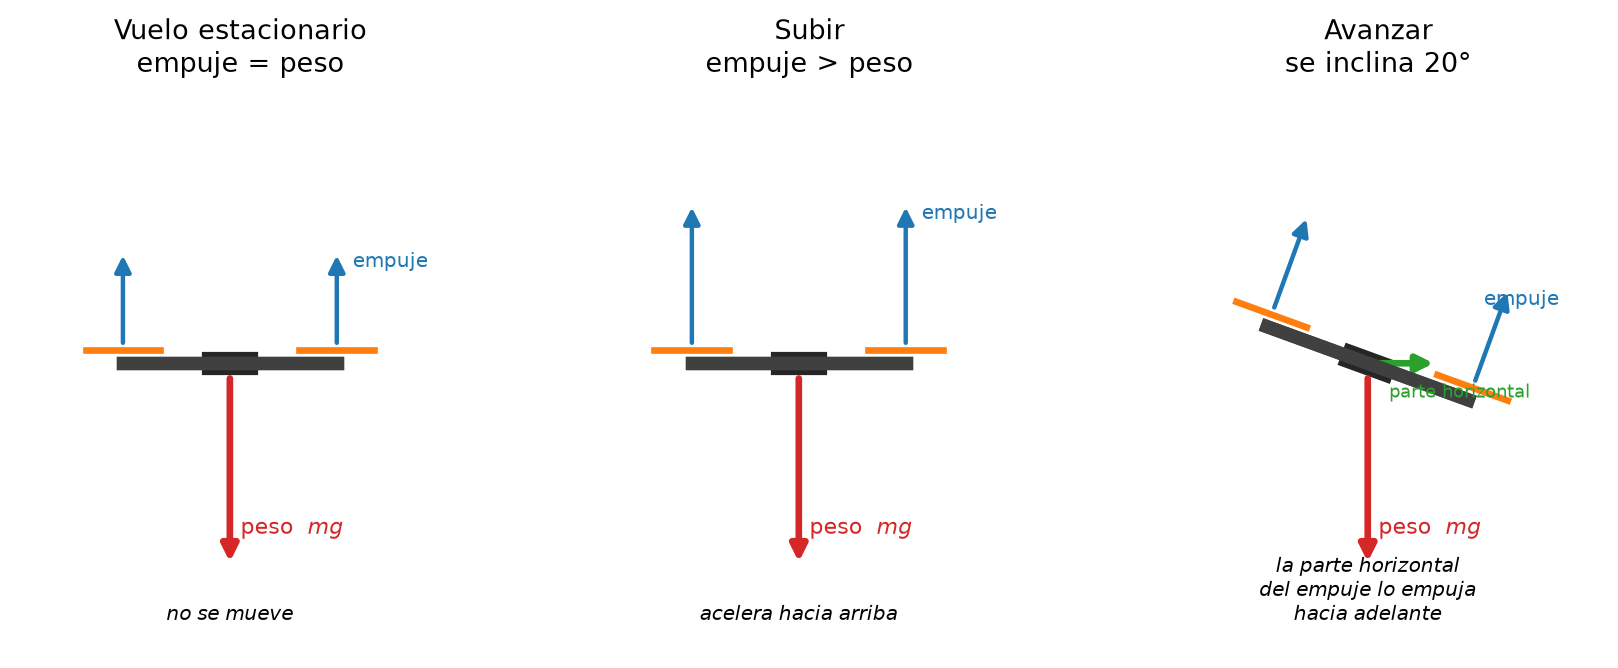
\includegraphics[width=\textwidth]{c_fuerzas.png}
\caption{Las dos fuerzas principales: el empuje de las hélices (azul) y el peso (rojo).}
\label{fig:fuerzas}
\end{figure}

\begin{itemize}
  \item Si el empuje total es igual al peso, el dron se queda quieto en el aire: \textbf{vuelo
        estacionario} (\emph{hover}).
  \item Si es mayor, sube; si es menor, baja.
  \item Para avanzar, el dron \textbf{se inclina}: el empuje ya no apunta hacia arriba, y su parte
        horizontal lo empuja hacia adelante (figura~\ref{fig:fuerzas}, derecha). Un cuadrirrotor no
        tiene ``motor hacia adelante'': avanza inclinándose, como una persona que se inclina para
        empezar a caminar.
\end{itemize}

\begin{ejemplo}
Sostén un libro con la mano extendida, plano. Para moverlo hacia adelante sin empujarlo, inclínalo un
poco: la fuerza de tu mano ``hacia arriba'' ahora tiene una parte hacia adelante. Así avanza un dron.
\end{ejemplo}

\section{Cómo se mueve: subir, alabeo, cabeceo y guiñada}

Un objeto en el espacio puede girar alrededor de tres ejes (figura~\ref{fig:ejes-c}). En aviación
esos giros tienen nombre:
\begin{description}
  \item[Alabeo (roll, $\phi$):] girar alrededor del eje que va al frente; el dron ``se ladea''.
  \item[Cabeceo (pitch, $\theta$):] girar alrededor del eje lateral; ``asiente con la cabeza''.
  \item[Guiñada (yaw, $\psi$):] girar alrededor del eje vertical; cambia hacia dónde mira.
\end{description}

\begin{figure}[H]
\centering
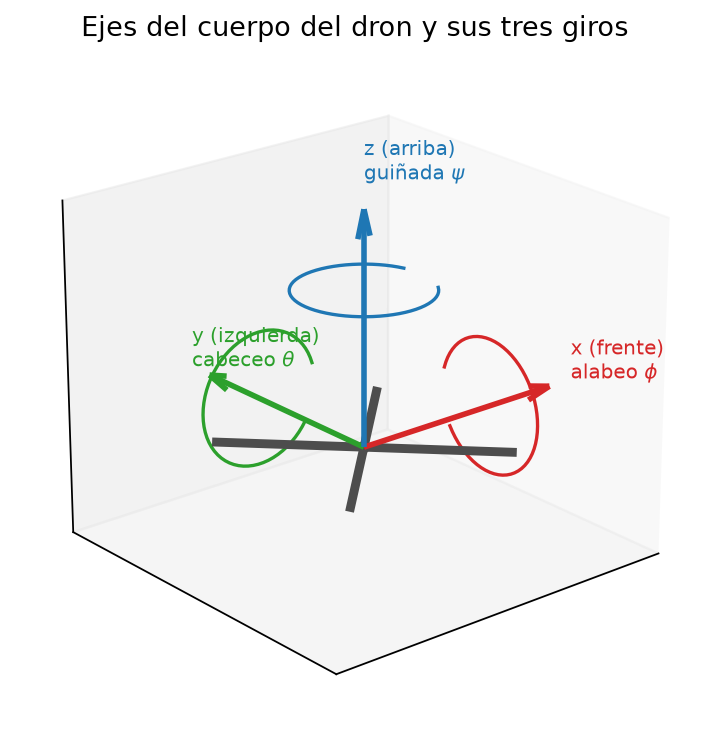
\includegraphics[width=0.6\textwidth]{c_ejes.png}
\caption{Ejes del cuerpo: \emph{x} al frente, \emph{y} a la izquierda, \emph{z} arriba.}
\label{fig:ejes-c}
\end{figure}

Con cuatro motores se controla todo así (figura~\ref{fig:movimientos}):

\begin{figure}[H]
\centering
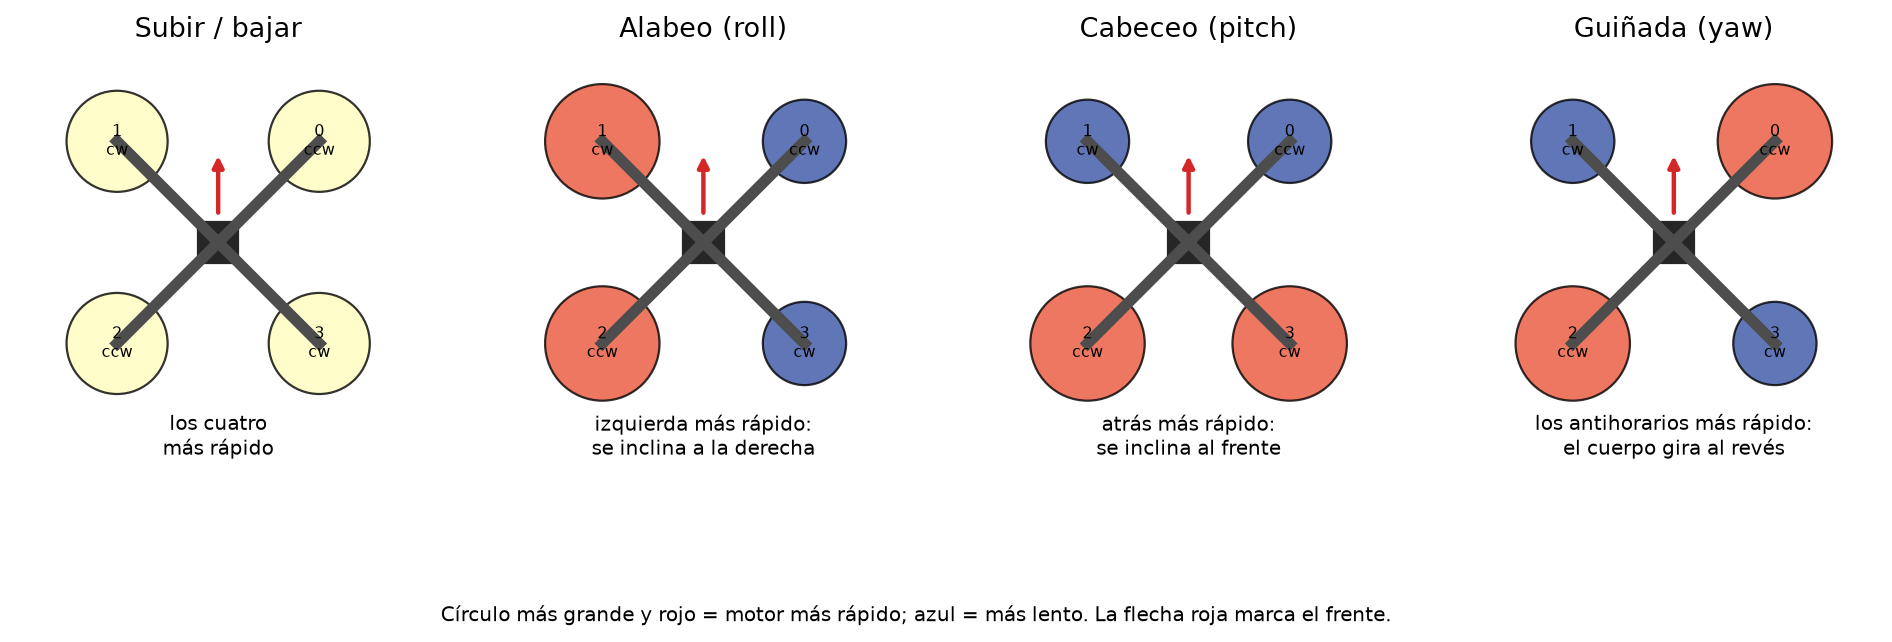
\includegraphics[width=\textwidth]{c_movimientos.png}
\caption{Cómo produce el dron cada movimiento solo cambiando la velocidad de los motores.}
\label{fig:movimientos}
\end{figure}

\begin{itemize}
  \item \textbf{Subir o bajar:} los cuatro motores aceleran o frenan por igual.
  \item \textbf{Alabeo:} los motores de un lado giran más rápido que los del otro; el dron se inclina
        hacia el lado lento y empieza a moverse de lado.
  \item \textbf{Cabeceo:} igual, pero adelante contra atrás; así avanza o retrocede.
  \item \textbf{Guiñada:} aquí entra un truco. Cada hélice, al girar, ``empuja'' el aire de lado y
        el aire, por reacción, intenta hacer girar al dron al revés. Por eso dos hélices giran en un
        sentido y dos en el otro: los efectos se cancelan. Si se aceleran las dos que giran en un
        sentido y se frenan las otras dos, el empuje total no cambia pero sobra par en un sentido, y
        el dron gira sobre sí mismo.
\end{itemize}

\begin{recuerda}
Cuatro motores, cuatro ``perillas'': empuje total, alabeo, cabeceo y guiñada. El avance y el
movimiento lateral no se controlan directamente: se consiguen inclinando el dron. Por eso el control
de un dron es \emph{en cascada}: para ir a una posición hay que pedir una inclinación, y para lograr
la inclinación hay que pedir velocidades a los motores.
\end{recuerda}

\section{Configuración ``+'' y ``X''}

Si un brazo apunta al frente, la configuración es ``+''; si el frente queda entre dos brazos, es
``X''. La ``X'' es la más común: la cámara frontal no ve hélices y los cuatro motores trabajan al
inclinarse hacia adelante. En la simulación hay un cuadrirrotor genérico en ``+'' y el Tarot en ``X''.

\section{El Tarot Ironman 650}

\begin{figure}[H]
\centering
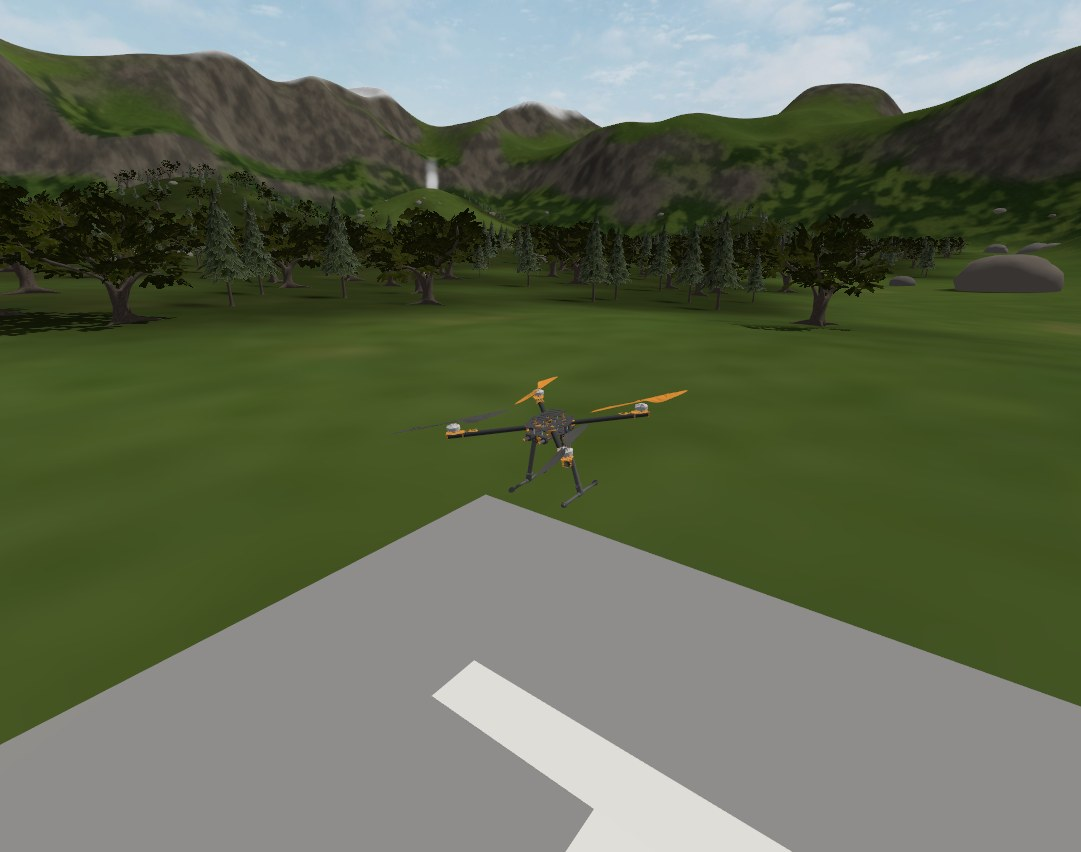
\includegraphics[width=0.8\textwidth]{gz_tarot_cerca.jpg}
\caption{El Tarot 650 simulado, en vuelo estacionario sobre su base.}
\end{figure}

El Tarot Ironman 650 es un marco comercial de fibra de carbono, muy usado en investigación porque
carga cámaras y computadoras sin problema. ``650'' es la distancia en milímetros entre motores
opuestos (en diagonal). Nuestro modelo:
\begin{itemize}
  \item motores a $(\pm0.22, \pm0.21)$~m del centro, en ``X'';
  \item hélices de 15'';
  \item 2.2~kg de masa total (supuesto);
  \item cada motor da hasta $\approx$19.6~N (unos 2~kg) de empuje: en total puede levantar
        $\approx$3.6 veces su peso. Esa \textbf{relación empuje/peso} da margen para maniobrar y
        resistir el viento.
\end{itemize}

\begin{tecnico}
En vuelo estacionario cada motor sostiene un cuarto del peso: $2.2\times9.81/4 = 5.4$~N. Como el
empuje es $f = k_f\omega^2$, con $k_f = 4.24\times10^{-5}$ la velocidad necesaria es
$\omega = \sqrt{5.4/k_f} = 357$~rad/s, unas 3400 revoluciones por minuto.
\end{tecnico}

\section{Para qué sirve un dron en un incendio forestal}

Un incendio se combate mejor cuanto antes se detecta y cuanto mejor se conoce su ubicación. Un dron
puede recorrer zonas de difícil acceso, ver por encima de las copas, detectar el humo desde lejos,
dar las coordenadas exactas del foco y quedarse vigilándolo, sin poner en riesgo a un piloto. Para
hacerlo de forma autónoma necesita tres capacidades, que son las tres partes centrales del libro:
\begin{enumerate}
  \item \textbf{Control} preciso aunque haya viento (Parte~II);
  \item \textbf{percepción}: ver y reconocer el fuego (Parte~III);
  \item \textbf{autonomía}: decidir a dónde ir y qué hacer (Parte~V).
\end{enumerate}
